%% REPLACE SXXXXXX with your student number
\def\studentNumber{SXXXXXX}


%% START of YOUR ANSWERS
%% Add answers to the questions below, by replacing the text inside the brackets {} for \youranswer{ "Text to be replaced with your answer." }. 
%
% Do not delete the commands for adding figures and tables. Instead fill in the missing values with your experiment results, and replace the images with your own respective figures.
%
% You can generally delete the placeholder text, such as for example the text "Question Figure 2 - Replace the images ..." 
%
% There are 18 TEXT QUESTIONS (a few of the short first ones have their answers added to both the Introduction and the Abstract). Replace the text inside the brackets of the command \youranswer with your answer to the question.
%
% There are also 3 "questions" to replace some placeholder FIGURES with your own, and 3 "questions" asking you to fill in the missing entries in the TABLES provided. 
%
% NOTE! that questions are ordered by the order of appearance of their answers in the text, and not by the order you should tackle them. Specifically, you cannot answer Questions 2, 3, and 4 before concluding all of the relevant experiments and analysis. Similarly, you should fill in the TABLES and FIGURES before discussing the results presented there. 
%
% NOTE! If for some reason you do not manage to produce results for some FIGURES and TABLES, then you can get partial marks by discussing your expectations of the results in the relevant TEXT QUESTIONS (for example Question 8 makes use of Table 1 and Figure 2).
%
% Please refer to the coursework specification for more details.


%% - - - - - - - - - - - - TEXT QUESTIONS - - - - - - - - - - - - 



%% Question 1:
\newcommand{\questionOne} {
    \youranswer{After each epoch of training, every batch of the dataset is forward propogated through the neural network model and then evaluated against the associated target labels through the error (or objective function) used for training the model, the final value of the error for model against the entire dataset is then given as the proportion of the cumulative error for each batch against the number of batches, this gives the error for each epoch of the training process. The accuracy for each epoch of training is calculated similarly to the error, except that we calculate the accuracy by taking the predicted classes given by the maximum logit of the output layer for each of the forward propogated data entries of the batch, then evaluate them against the true associated classes and taking the mean as the accuracy for each batch, then just as was done with the error, the final accuracy is given as the average over the entire batch. Both plots present the error and accuracies over the total epochs.



    We can see that at around the 10\textsuperscript{th} epoch, the error of the model for the validation dataset is at its minimum, it then begins to curve upwards this upward curvature is exactly where the overfitting occurs and is due to the model fitting too well to the training dataset (resulting in the variance of the models prediction with respect to the underlying distribution being very high), meaning it has become sensitive to the noise of the data.

    




The Figure 1 presents the error and accuracy evaluations of a neural network being trained on the data, the accuracy is given by the ratio of correctly predicted labels against the total dataset, the graph provides a running accuracy and error over each training cycle (the Epoch), for both the validation and validation datasets..}
}

%% Question 2:
\newcommand{\questionTwo} {
\youranswer{Question 2 - Present your network width experiment results by using the relevant figure and table}
}

%% Question 3:
\newcommand{\questionThree} {
\youranswer{Question 3 - Discuss whether varying width affects the results in a consistent way, and whether the results are expected and match well with the prior knowledge (by which we mean your expectations as are formed from the relevant Theory and literature)

}
}

%% Question 4:
\newcommand{\questionFour} {
\youranswer{Question 4 - Present your network depth experiment results by using the relevant figure and table}
}

%% Question 5:
\newcommand{\questionFive} {
\youranswer{Question 5 - Discuss whether varying depth affects the results in a consistent way, and whether the results are expected and match well with the prior knowledge (by which we mean your expectations as are formed from the relevant Theory and literature)

}
}


%% Question 6:
\newcommand{\questionSix} {
\youranswer{Question 6 - Explain how one could use a combination of L1 and L2 regularisation. Discuss any potential benefits of this approach. Present an equation for this combined loss function and explain all relevant variables and hyperparameters.}

$$
- \log p_\theta \big( y^{(i)} \mid x^{(i)} \big)
=
- z_\theta(x^{(i)})_{y^{(i)}} 
+ 
\log \Bigg(
\sum_{j=1}^{K}
\exp \big( z_\theta(x^{(i)})_j \big)
\Bigg).
$$

}


%% Question 7:
\newcommand{\questionSeven} {
\youranswer{Question 7 - Assume you had a limited experiment budget for exactly \textbf{4} experiment runs dedicated to testing the effectiveness of your proposed combination of L1 and L2 Regularization in Section~\ref{sec:L1L2combo}. Argue for which 4 configurations to run based on any previous results or other information you consider relevant. Run those experiments and add the results in Table~4 and Figure~5 (you will then discuss those results alongside all others in the next question below).

(Even if you have not managed to implement your L1 and L2 combination; still argue based on your proposed approach).

    The L$1$ and L$2$ penalty are calculated for all of the weights and bias vectors in the model, in our implementation the penalty was applied to each layer during the training phase only, by simply adding the value of the gradient of the penalty elementwise to the gradients of the loss function with respect to each weight (the same was done for the bias vector). These penalties have different effects on the behaviour of the gradient descent algorithm during training, we can examine this in a more simple case using their derivates. Each iteration of the (non-stochastic) gradient descent algorithm for a single weight parameter is given as ${w}_i = {w_{i-1}} - \epislon \nabla f(x)$ where $f(x)$ is the objective function, the algorithm converges as $\nabla f(x) \to 0$, therefore given that $\nabla f(x) = \frac{\delta L}{\delta w_i} + \lambda \sign(w_i) \to 0$, for this function to be as close to 0 as possible, we could reduce the magnitude of the gradient term using $\lambda$ term, in which case a choice of the sign of the weight that opposes the sign of the gradient is preferable, or we may choose for ${w_i}=0$ in the case that $\lambda$ is larger than the gradient. From our previous derivation of the loss function gradient with respect to the input layer weights \ref{eq:loss_gradient_cross_softmax} we can see that the size of each element of the input as well as the prediction error has a direct effect on the magnitude of this gradient, therefore it would make sense that an optimal solution would involve a sparse set of weights, where the value of the weights that contribute little to the gradient of the loss function will be zero. For the L$2$ penalty we have a different effect, the gradient of a singular weight for this penalty is given by $\lambda w_i$, therefore if we rearrange the expression we obtain ${w}_i = -\frac{1}{\lambda}\frac{\delta L}{\delta \mathcal{w}_i}$, therefore this penalty causes all of the weights to be closer to zero.
    

    Therefore, we chose 4 permutations of parameters that produced the most accurate models in either of the penalties cases. Table 4 illustrates the results.
}
}


%% Question 8:
\newcommand{\questionEight} {
\youranswer{Question 8 - Explain the experimental details (e.g. hyperparameters), discuss the results in terms of their generalisation performance and overfitting. Select and test the best performing model as part of this analysis.
    % The results of the dropout based model also make it very clear that number of parameters of the neural network is only slightly redundant for the given data, since the model beats the baseline at a high inclusion probability starting from $p=0.85$, this is evidence that the model is overfitting to the training data, however that the majority of the parameters of the model are necessary in order to make accurate predictions.

    A matrix (or vector) norm is a metric for its size, given that the optimisation problem that our stochastic gradient descent aglroithm is trying to solve is that of a minimisation one, this means that this penalty results in weights of greater accumulative size being penalised over those of smaller sizes, therefore the coefficient for the penalty of both norms is proportional to the amount that the weights are restricted to being of a smaller value.

    In table 4, the first noticeable result is the results of the L$1$ penalty, there is a large difference in validation accuracy between the neural networks with the L$1$ penalty of values $0.001$ and $0.005$, from our previous paragraph analysing the nature of the L$1$ penalty, we may conclude that the inputs and weights of the model have a great effect on its accuracy, as the small increase in the value of the coefficient (which would cause the zeroing of parameters in the model) has caused a massive decrease in accuracy. This is made more obvious by the improvement of the neural network with L$2$ penalty against the baseline, this means that a reduction in the magnitude of all weights has improved the accuracy of the model. From this we can conclude that the contribution of every distinct pixel in the image are of importance, which makes sense, given that the information available for classifying an image is given by the pixels that make up that image.


    
    

}
}


%% Question 9:
\newcommand{\questionNine} {
\youranswer{Question 9 - A colleague proposed using a custom activation function (which can be identified as CustomActivationLayer() in your Coursework\_1.ipynb notebook and the mlp package). Run the prepared experiment in the "Problematic Training" cell in your Coursework\_1.ipynb notebook, and display the results in Figure~6. Analyse the results. Is the model overfitting? Explain the cause of the problematic performance of the model?

    The custom activation function used in this model is scaled logistic function scaled by a constant coefficient, it is defined as $$\frac{1}{20} \sigma(x) = \frac{1}{20(1+\exp(-x))},$$ the original range of this function was $(0,1)$ therefore the scaled logistic function would therefore have the range $(0,0.05)$. We can see evidence of the true issue in the gradient flow graph of Figure ..., which shows an average gradient of zero at the layers the correspond to this custom logistic function, this problem is known as the vanishing gradient problem and is caused by an issue in the calculation of gradients in the backpropogation algorithm \cite{hochreiterGradientFlowRecurrent2001}. For backpropogation, the gradient of the loss with respect to the weights for a layer $l$ is given by $$\Delta_{w^{l}} L = \alpha^{(l+1)} \sigma(x^l)^T$$, where $\sigma$ is the activation function and $\alpha^{l}$ is the error signal computed at each stage by the backpropogation algorithm and is given by $$\alpha^{(l)} = \prod_{k=l}^{L-1} J_{\sigma}(z^{(k)}) (W^{(k+1)})^T \alpha^{(L)}$$ where $L$ is the index of the final layer \cite{petersenMathematicalTheoryDeep2025}.

    Therefore for this specific activation function, the error signal would be given by $$\alpha^{(l)} = \left(\frac{1}{80} \right)^{L-l} \prod_{k=l}^{L-1} J_{\sigma}(z^{(k)}) (W^{(k+1)})^T \alpha^{(L)}$$, as we can see from the coefficient term this would result in an asymptotic decay for each subsequent layer of weights of order $O(80^{-n})$.

    Given that the gradient would then be very small, the perturbation of the weights by stochastic gradient descent will consequently also be small, resulting in a prohibitively slow training process. Knowing we have initialised our weights using Glorot initialisation \cite{glorotUnderstandingDifficultyTraining2010} (resulting in the average of the weights being zero), we can see can see from the gradient flow graph our exact hypothesis, that the change in the mean gradient of the weights has been minimal as the average gradient for every layer other than the final layer (with no subsequent custom residual layer) has an average gradient of approximately zero. 

    % One method for addressing this problem whilst keeping the type of activation function is to instead implement it as a residual activation function \cite{heDeepResidualLearning2015}, this method 

    % in the backpropogation algorithm, the gradient of the loss function with respect to the weights for a layer $l$ (which is used in the stochastic gradient descent to update them) is dependent upon a product of the jacobian of the activation functions of each subsequent layer, for this custom logistic function the jacobian is a diagonal matrix whose elements are given by $$$J_\sigma(x^l) = \diag{\frac{1}{20}(\sigma(x^l)(1 - 20\sigma(x^l)))}$$, given the spectral norm of this jacobian matrix is $\|J_\sigma(x)\| = \frac{1}{80}$ this means that we have an exponential decline of order $O(0.0125^n)$ for each subsequent logistic activation layer. 
    % The custom activation function is a logistic activation function $\frac{1}{20} \sigma(x)$ with a rational constant coefficient, we can see the issue causing the very low accuracy by looking at the average gradient of each layer, as we can see from the gradient flow graph of figure 6, at layer 9, which corresponds to the pass of the gradients of the loss with respect to the weights through the custom logistic activation layer, the average value of the gradients decreases significantly towards 0, furthermore, we can see after this that for each step in the backpropogation algorithm, if the layer is a custom activation layer the average gradient is 0, whereas if it is an affine layer it is slightly above 0, although with each epoch this diminishes towards 0. This is known as the vanishing gradient problem, it occurs as a result of the calculation of the gradients of each layer being given by the product of the gradients of the previous layers, if those gradients are all below 1, then this product tends towards 0 and the gradient vanishes. 

    % Therefore the model is not overfitting, instead this is an issue with the flow of gradients through the neural network layers during backpropogation, the cause of this issue is a result of the way that the  is backpropogated through the network \cite{Hochreiter} (which studied this for RNN\'s, however the same principle applies here in terms of layers), the gradient of each logistic activation layer for the loss with respect to the weights of layer $l$ can be given by $$\frac{\delta L}{\delta W^l} = \delta{(l)}a^(l-1)$$ where $a^{(l-1)}$ is the ouput of the previous layer and $\delta^{l}$ is known as the error signal which is computed as $$\delta^{(l)} = J_\sigma (x^{l})(W^{l})^T \delta^{(l+1)}$$, now given that for this logistic acitvation function the jacobian is the diagonal matrix with elements given by $\sigma'(x_{ij}) = \sigma(x_{ij})(1-20\sigma(x_{ij}))$




}
}




%% Question 10:
\newcommand{\questionTen} {
\youranswer{Question 10 - Briefly draw your conclusions based on the results from the previous sections (what are the take-away messages?), discussing them in the context of the overall literature, and conclude your report with a recommendation for future directions



}
}

%% - - - - - - - - - - - - FIGURES - - - - - - - - - - - - 

%% Question Figure 2:
\newcommand{\questionFigureTwo} {
\youranswer{Question Figure 2 - Replace the images in Figure 2 with figures depicting the accuracy and error, training and validation curves for your experiments varying the number of hidden units.
%
\begin{figure}[t]
    \centering
    \begin{subfigure}{\linewidth}
        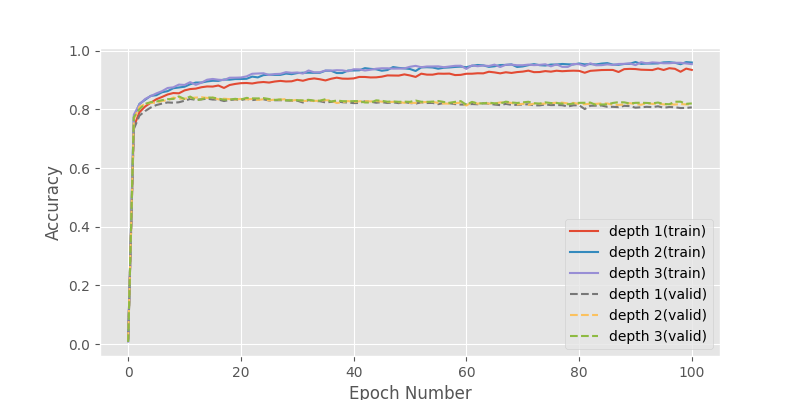
\includegraphics[width=\linewidth]{figures/acc_curve_width.png}
        \caption{accuracy by epoch}
        \label{fig:width_acccurves}
    \end{subfigure} 
    \begin{subfigure}{\linewidth}
        \centering
        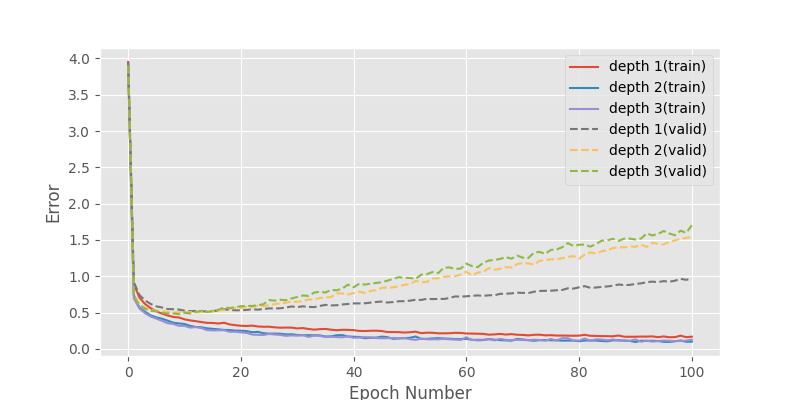
\includegraphics[width=\linewidth]{figures/error_curve_width.png}
        \caption{error by epoch}
        \label{fig:width_errorcurves}
    \end{subfigure} 
    \caption{Training and validation curves in terms of classification accuracy (a) and cross-entropy error (b) on the EMNIST dataset for different network widths.}
    \label{fig:width}
\end{figure} 
}
}

%% Question Figure 3:
\newcommand{\questionFigureThree} {
\youranswer{Question Figure 3 - Replace these images with figures depicting the accuracy and error, training and validation curves for your experiments varying the number of hidden layers.
%
\begin{figure}[t]
    \centering
    \begin{subfigure}{\linewidth}
        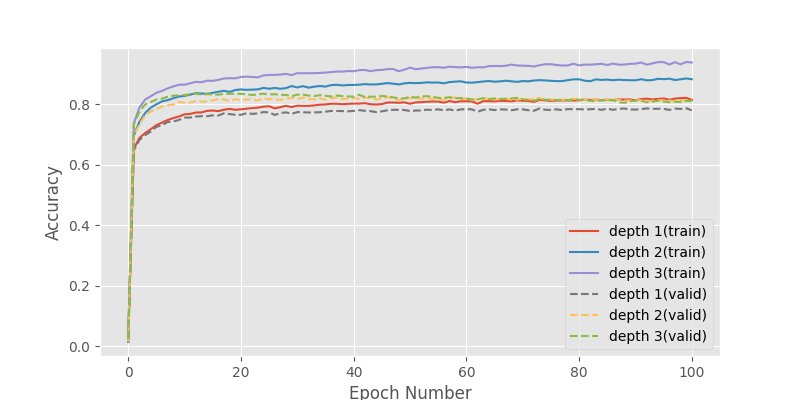
\includegraphics[width=\linewidth]{figures/acc_curve_depth.png}
        \caption{accuracy by epoch}
        \label{fig:depth_acccurves}
    \end{subfigure} 
    \begin{subfigure}{\linewidth}
        \centering
        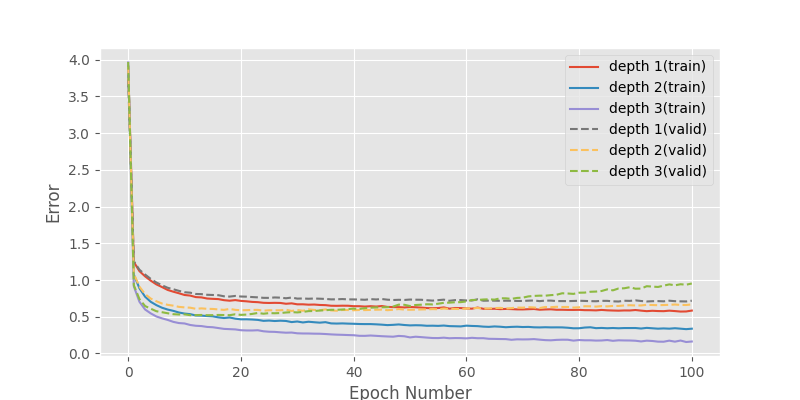
\includegraphics[width=\linewidth]{figures/error_curve_depth.png}
        \caption{error by epoch}
        \label{fig:depth_errorcurves}
    \end{subfigure} 
    \caption{Training and validation curves in terms of classification accuracy (a) and cross-entropy error (b) on the EMNIST dataset for different network depths.}
    \label{fig:depth}
\end{figure} 
}
}

%% Question Figure 4:
\newcommand{\questionFigureFour} {
\youranswer{Question Figure 4 - Replace these images with figures depicting the Validation Accuracy and Generalisation Gap (difference between validation and training error) for each of the experiment results varying the Dropout inclusion rate, and L1/L2 weight penalty depicted in Table 3 (including any results you have filled in).
%
\begin{figure*}[t]
    \centering
    \begin{subfigure}{.475\linewidth}
        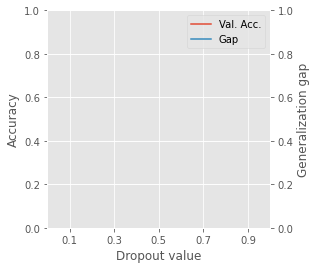
\includegraphics[width=\linewidth]{figures/empty_dropout_plot.png}
        \caption{Accuracy and error by inclusion probability.}
        \label{fig:dropoutrates}
    \end{subfigure} 
    \begin{subfigure}{.475\linewidth}
        \centering
        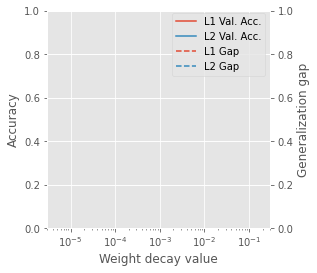
\includegraphics[width=\linewidth]{figures/empty_wd_plot.png}
        \caption{Accuracy and error by weight penalty.}
        \label{fig:weightrates}
    \end{subfigure} 
    \caption{Accuracy and error by regularisation strength of each method (Dropout and L1/L2 Regularisation).}
    \label{fig:hp_search}
\end{figure*}
}
}

%% Question Figure 5:
\newcommand{\questionFigureFive} {
\youranswer{Question Figure 5 - Add figures depicting the Validation Accuracy and Generalisation Gap (difference between validation and training error) for each of your 4 experiments  varying your hyperparameters for the combination of L1 and L2 regularisation (based on your implementation) depicted in Table 4.
}
}

%% Question Figure 6:
\newcommand{\questionFigureSix} {
\youranswer{Question Figure 6 - Add figures depicting the Training Accuracy, Error, and Gradient Flow Across Layers for the 1 experiment run with the Custom Activation function (produce these by running the "Problematic Training" cell in the Coursework\_1.ipynb notebook).
}
}

%% - - - - - - - - - - - - TABLES - - - - - - - - - - - - 

%% Question Table 1:
\newcommand{\questionTableOne} {
\youranswer{
Question Table 1 - Fill in Table 1 with the results from your experiments varying the number of hidden units.
%
\begin{table}[t]
    \centering
    \begin{tabular}{c|ccc}
    \toprule
        \# Hidden Units & Val. Acc. & Train Error & Val. Error\\
    \midrule
         32            &    77.9   &  0.584 &   0.719            \\
         64            &    81.1   &  0.338  &   0.668               \\
         128           &    80.9   &  0.163  &   0.953           \\ 
    \bottomrule
    \end{tabular}
    \caption{Validation accuracy (\%) and training/validation error (in terms of cross-entropy error) for varying network widths on the EMNIST dataset.}
    \label{tab:width_exp}
\end{table}
}
}

%% Question Table 2:
\newcommand{\questionTableTwo} {
\youranswer{
Question Table 2 - Fill in Table 2 with the results from your experiments varying the number of hidden layers.
%
\begin{table}[t]
    \centering
    \begin{tabular}{c|ccc}
    \toprule
        \# Hidden Layers & Val. Acc. & Train Error & Val. Error \\
    \midrule
         1               &      80.7      &   0.167 & 0.967                \\
         2               &      81.7      &   0.099 & 1.542                \\
         3               &      82.0      &   0.126 & 1.701                \\ 
    \bottomrule
    \end{tabular}
    \caption{Validation accuracy (\%) and training/validation error (in terms of cross-entropy error) for varying network depths on the EMNIST dataset.}
    \label{tab:depth_exps}
\end{table}
}
}

%% Question Table 3:
\newcommand{\questionTableThree} {
\youranswer{
Question Table 3 - Fill in Table 3 with the results from your experiments for the missing hyperparameter values for each of L1 regularisation, L2 regularisation, Dropout and label smoothing (use the values shown on the table).
%
\begin{table*}[t]
    \centering
    \begin{tabular}{c|c|ccc}
    \toprule
        Model    &  Hyperparameter value(s) & Validation accuracy & Train Error & Validation Error \\
    \midrule
    \midrule
        Baseline &  -                    &               83.7 &       0.241 &  0.533          \\
    \midrule
        \multirow{4}*{Dropout}
                 & 0.6                   &  80.7                &      0.549 & 0.593     \\
                 & 0.7 & 83.9 & 0.349 & 0.476  \\
                 & 0.85 & 85.1 &  0.329 &  0.434 \\
                 & 0.97 & 85.4 &  0.244 & 0.457  \\
    \midrule
        \multirow{4}*{L1 penalty}
                 & 5e-4 & 79.5 & 0.642 & 0.658 \\
                 & 1e-3 & 75.9 & 0.772 & 0.788 \\
                 & 5e-3 & 2.41 & 3.850 & 3.850 \\
                 & 5e-2 & 2.20 & 3.850 & 3.850 \\
    \midrule
        \multirow{4}*{L2 penalty}  
                 & 5e-4 & 85.1 & 0.306 & 0.460 \\
                 & 1e-3 & 85.4 & 0.364 & 0.432 \\
                 & 5e-3 & 81.3 & 0.586 & 0.607 \\
                 & 5e-2 & 39.2 & 2.258 & 2.256  \\
    \midrule
        Label smoothing & 0.1 & 83.2 & 0.850 & 1.234 \\
    \bottomrule
    \end{tabular}
    \caption{Results of all hyperparameter search experiments. \emph{italics} indicate the best results per series (Dropout, L1 Regularisation, L2 Regularisation, Label smoothing) and \textbf{bold} indicates the best overall.}
    \label{tab:hp_search}
\end{table*}
}
}


%% Question Table 4:
\newcommand{\questionTableFour} {
\youranswer{
Question Table 4 - Add a table with the results from your 4 experiments (by which we mean: 4 training runs, NOT 4 sets of experiments) varying your hyperparameters for the combination of L1 and L2 regularisation (based on your implementation).
}
}

%% END of YOUR ANSWERS
